%%%%%%%%%%%%%%%%%%%%%%%%%%%%%%%%%%%%%%%%%
% Short Sectioned Assignment
% LaTeX Template
% Version 1.0 (5/5/12)
%
% This template has been downloaded from:
% http://www.LaTeXTemplates.com
%
% Original author:
% Frits Wenneker (http://www.howtotex.com)
%
% License:
% CC BY-NC-SA 3.0 (http://creativecommons.org/licenses/by-nc-sa/3.0/)
%
%%%%%%%%%%%%%%%%%%%%%%%%%%%%%%%%%%%%%%%%%

%----------------------------------------------------------------------------------------
%   PACKAGES AND OTHER DOCUMENT CONFIGURATIONS
%----------------------------------------------------------------------------------------

\documentclass[paper=letter, fontsize=11pt]{scrartcl} % A4 paper and 11pt font size
\synctex=1
\usepackage[T1]{fontenc} % Use 8-bit encoding that has 256 glyphs
\usepackage{fourier} % Use the Adobe Utopia font for the document - comment this line to return to the LaTeX default
\usepackage[english]{babel} % English language/hyphenation
\usepackage{amsmath,amsfonts,amsthm} % Math packages
%\usepackage[nolists, nomarkers]{endfloat}
\usepackage{hyperref}
\usepackage{bm}
\usepackage{graphicx}
\usepackage[section]{placeins}
\usepackage{sectsty} % Allows customizing section commands
\allsectionsfont{\normalfont\scshape} % Make all sections centered, the default font and small caps

\usepackage{fancyhdr} % Custom headers and footers
\pagestyle{fancyplain} % Makes all pages in the document conform to the custom headers and footers
\fancyhead{} % No page header - if you want one, create it in the same way as the footers below
\fancyfoot[L]{} % Empty left footer
\fancyfoot[C]{} % Empty center footer
\fancyfoot[R]{\thepage} % Page numbering for right footer
\renewcommand{\headrulewidth}{0pt} % Remove header underlines
\renewcommand{\footrulewidth}{0pt} % Remove footer underlines
\setlength{\headheight}{13.6pt} % Customize the height of the header

\numberwithin{equation}{section} % Number equations within sections (i.e. 1.1, 1.2, 2.1, 2.2 instead of 1, 2, 3, 4)
\numberwithin{figure}{section} % Number figures within sections (i.e. 1.1, 1.2, 2.1, 2.2 instead of 1, 2, 3, 4)
\numberwithin{table}{section} % Number tables within sections (i.e. 1.1, 1.2, 2.1, 2.2 instead of 1, 2, 3, 4)

\setlength\parindent{0pt} % Removes all indentation from paragraphs -
                          % comment this line for an assignment with
                          % lots of text
\setlength\parskip{12pt}


%----------------------------------------------------------------------------------------
%   TITLE SECTION
%----------------------------------------------------------------------------------------

\newcommand{\horrule}[1]{\rule{\linewidth}{#1}} % Create horizontal rule command with 1 argument of height

\title{ 
\normalfont \normalsize 
\textsc{Exoplanet Patchy Cloud Project} \\ [25pt] % Your university, school and/or department name(s)
\horrule{0.5pt} \\[0.4cm] % Thin top horizontal rule
\huge Cross Correlation Test and Preliminary Aperture Photometry Result\\ % The assignment title
\horrule{2pt} \\[0.5cm] % Thick bottom horizontal rule
}

\author{Yifan Zhou} % Your name

\date{\normalsize\today} % Today's date or a custom date

\begin{document}

\maketitle % Print the title
\section{Summary}
\begin{enumerate}
\item Using cross correlation, images can be aligned with precision of
  $\sim 0.01$ pixels, which is far better than the precision that IDL
  \texttt{cntrd.pro} and \texttt{gcntrd.pro} routines can
  provide. According to the patterns on PSF subtracted images, cross
  correlation has better performance tan WCS alignment.
\item Aperture photometry for secondary object in ABPIC system is
  carried out with a fixed aperture radius of 5 pixels. The light
  curves are very similar to Glenn's measurement. The light curves for
  two filters, F125W and F160W have better agreement in my
  measurement.
\item Taking only statistical uncertainty (counting error) and
  background fluctuations into account, a rough estimation gives an
  relative uncertainty of 0.3\% for one photometry measurement.
  
\end{enumerate}
\section{Image Registration}
\subsection{Image Registration Precision Test}
The performance of image registration method is valuated by the accuracy of
the measurement for shift between two images. In practice, I
choose one image, shift this image with a specific distance with
\texttt{fshift.pro}, measure the shift, and calculate the offset of
the measured shift and real shift. With above procedure, I tested the
performance of 3 image registration method. Results are plotted in figure \ref{fig:shift1}.\par

The offsets for cntrd and gcntrd methods can be as large as 0.2 - 0.3
pixels. However cross correlation method can limit the offset within
0.06 pixels. It is surprising that none of the three distributions of
offsets has a Gaussian like  profile. For cross correlation, I plotted
the offset against the real shift distance. It turned out that the
offset oscillates with shift distance with a period of exact 1 pixel
and an amplitude of 0.05 pixels. I do not know clearly why they have
such a relationship.\par

According to the test result, cross correlation has a much better
performance on registration images.

\begin{figure}
  \centering
  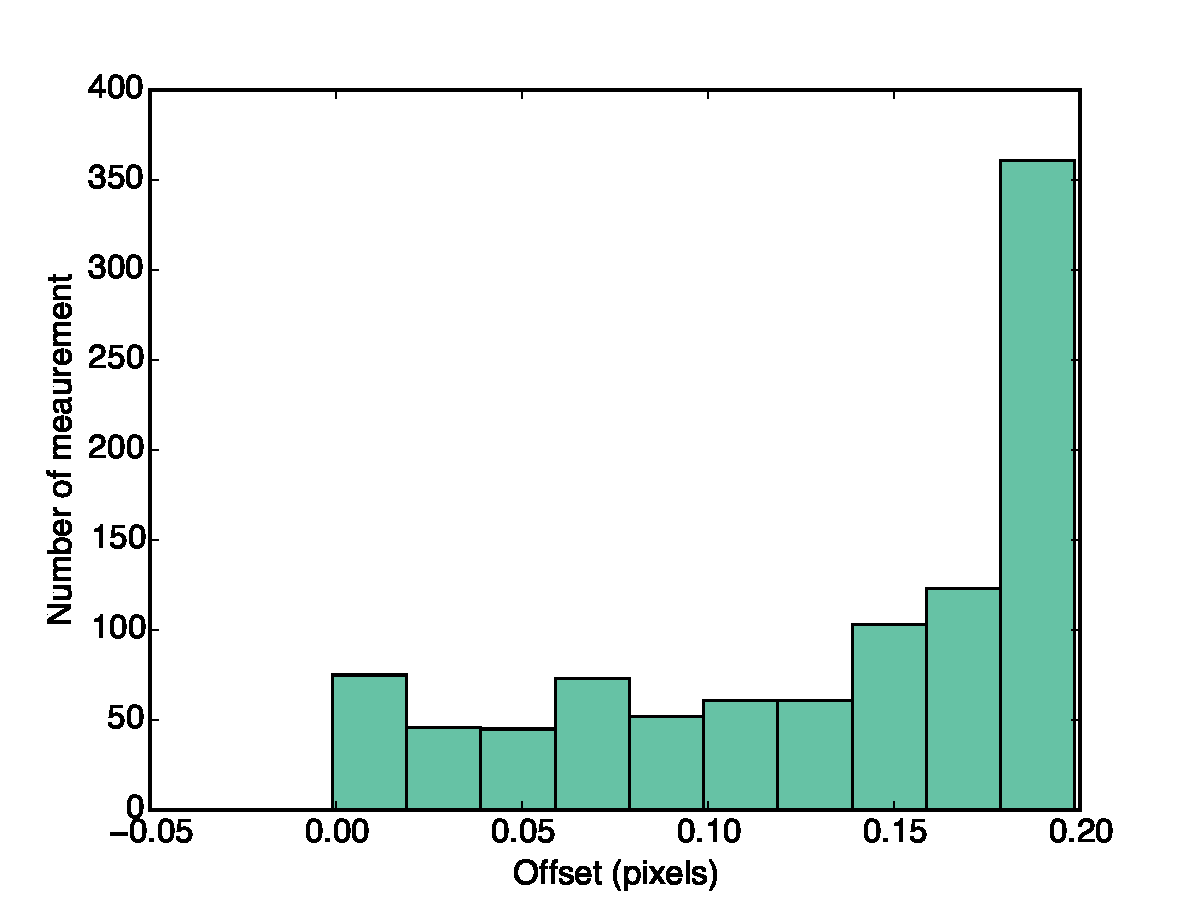
\includegraphics[width=0.48\textwidth]{cntrd_off2}
  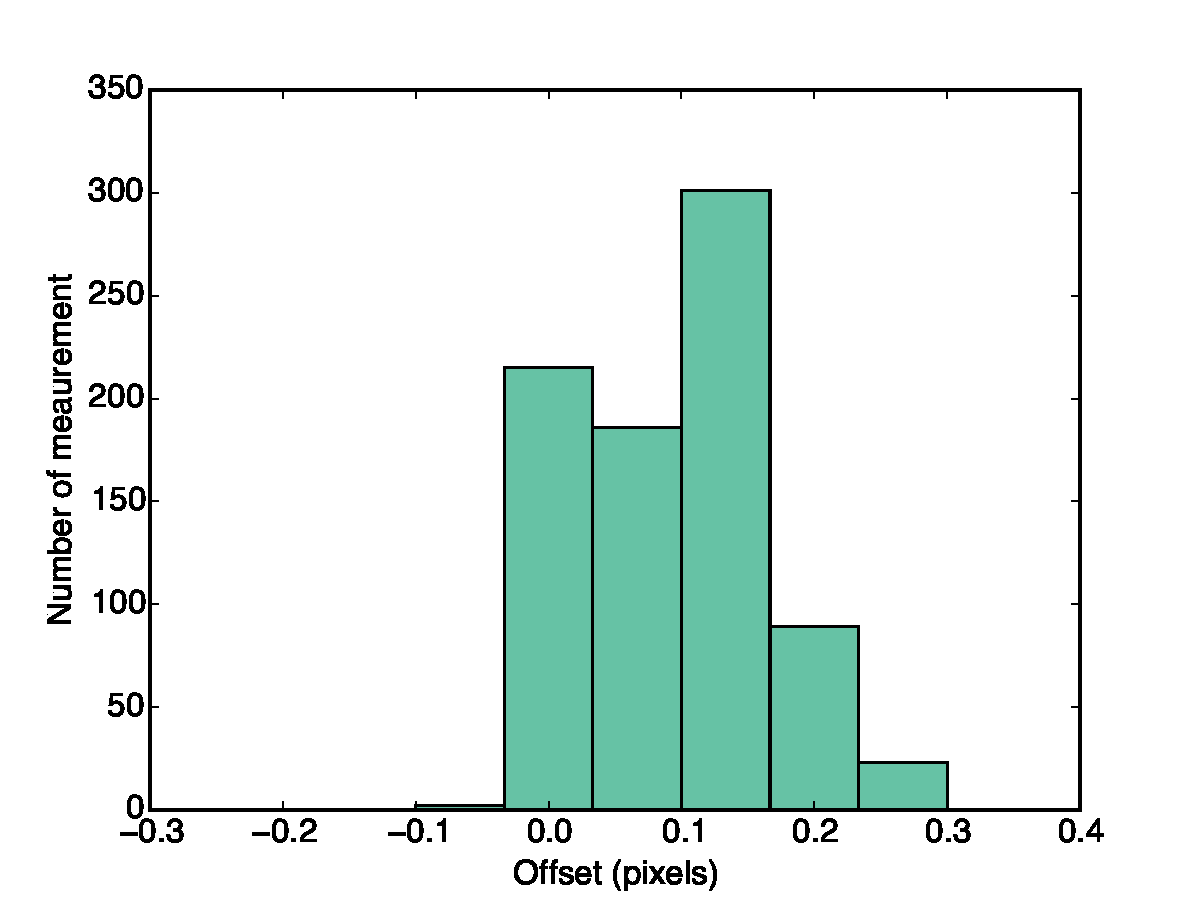
\includegraphics[width=0.48\textwidth]{gcntrd_off2}\\
  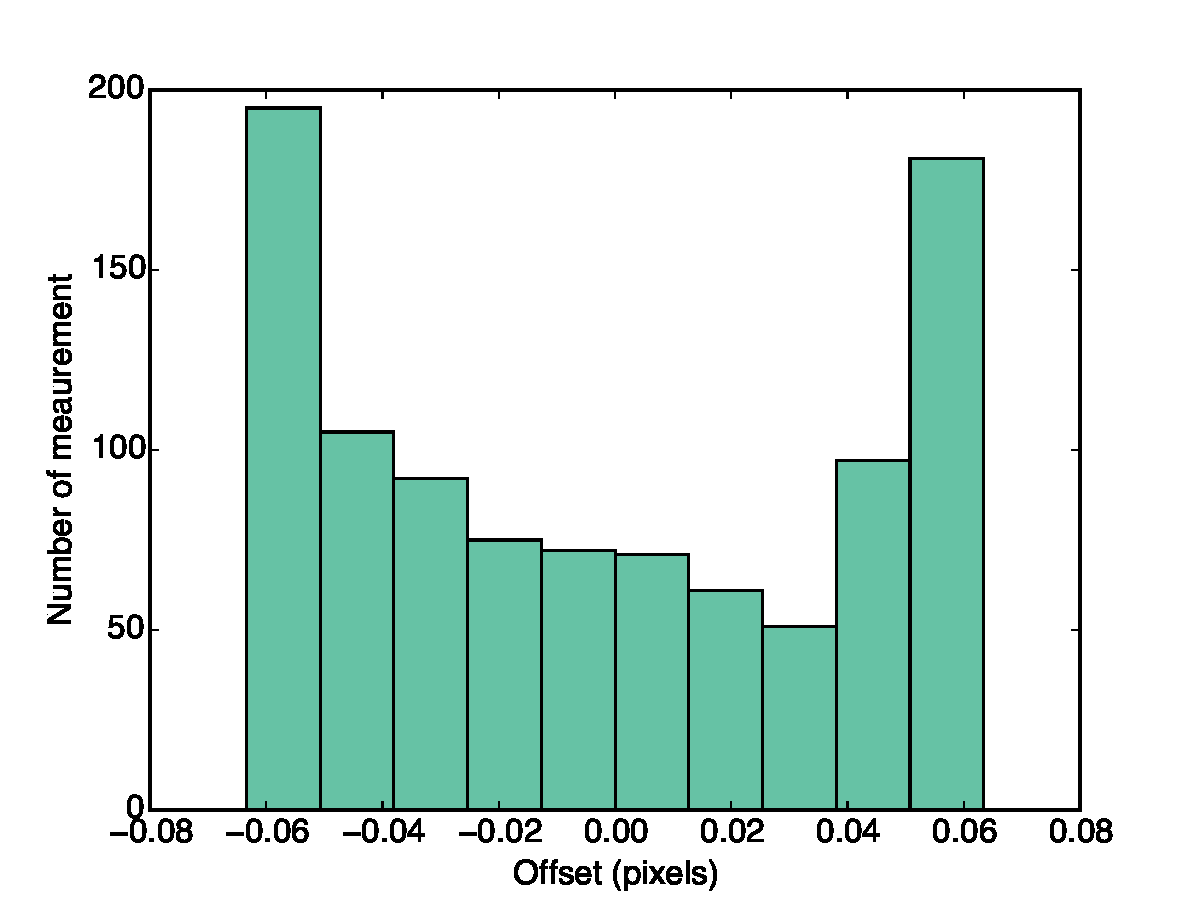
\includegraphics[width=0.48\textwidth]{crosscorr_off2}
  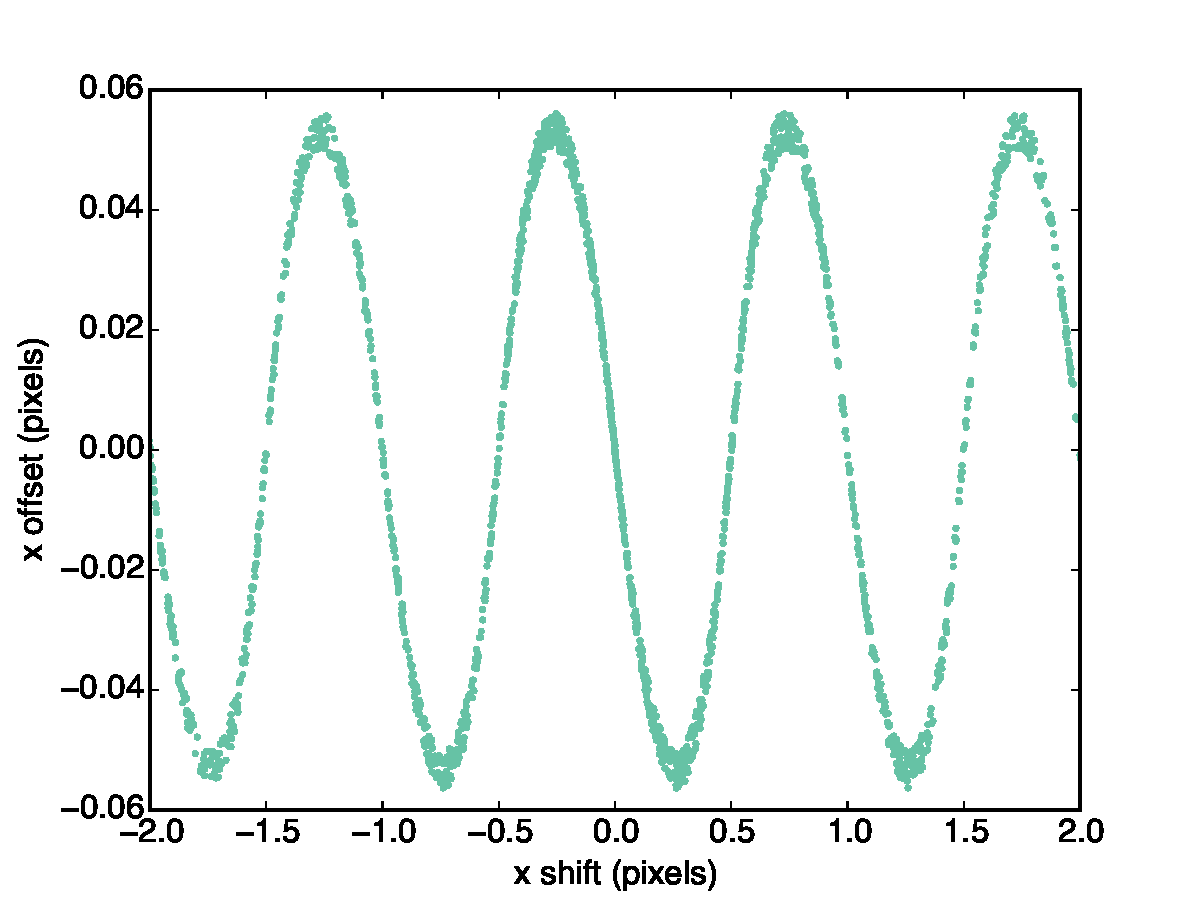
\includegraphics[width=0.48\textwidth]{crosscorr_cenTes.pdf}\\
  \caption{Measured shifts minus real shifts histogram in x direction
    measured by IDL \texttt{cntrd.pro} IDL \texttt{gcntrd.pro} and
    cross correlation}
  \label{fig:shift1}
\end{figure}

\subsection{Modification of  Cross correlation}
The general idea of cross correlation method is that it calculate
cross correlation matrix of one image and one reference image. The
coordinate of the maximum in cross correlation matrix then can be
converted to the shifts in x and y direction of the image  relative to
the reference image. To locate the peak in cross correlation matrix
is one key factor of the accuracy of this method. The original
\texttt{crosscorr.pro} routine use \texttt{polyfit2d.pro} to find the
maximum, which uses a polynomial function (default order is 4) to fit
the an area around the maximum value (default is a (5 pixel)$^{2}$
square) and find the peak. I tried to fit either with a higher order
or larger area, the result turned to be unstable. Especially, when I
kept on using an order of 4 polynomial function to fit a (10
pixel)$^{2}$ square around the peak, the program got stuck and
returned error.\par

Therefore, I tried \texttt{mpfit2dpeak.pro} routine which fits either
Gaussian, Lorentz or Moffat function to find the peak. It turned out
that  mpfit could improve the accuracy of cross correlation for
nearly an order of magnitude. With mpfit, the offset for measured
shift and real shift can be limited within 0.008 pixels. However, the
weird oscillation still exists.\par

\begin{figure}[h]
  \centering
  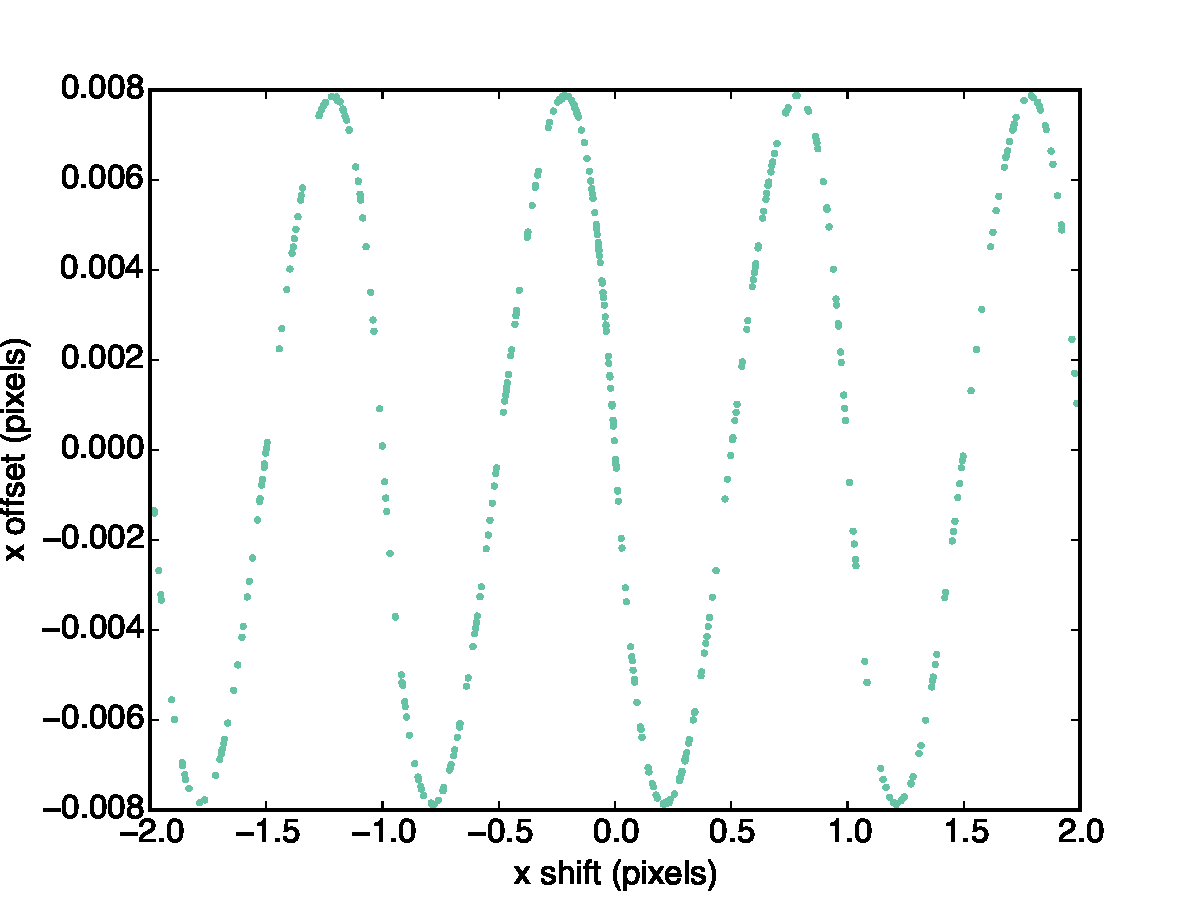
\includegraphics[width=0.8\textwidth]{crosscorr_cenTest2}
  \caption{offset for measured shift and real shift. The shift is measured by cross correlation with mpfit.}
\end{figure}

\subsection{Test with Noise Adding in}
Primary star image is subtracted with a PSF image that has a different
rolling angle. Thus it is important to know the accuracy in the
scenario  where only the primary star image stays the same, other
objects rolled to a specific angle. To simulate rolling, I add 5 fake
star images in random positions to both original image and shifted
image and then use cross correlation to measure the shift. As shown in
figure \ref{fig:shift2}, noise star images does not affect the
accuracy too much.

\begin{figure}[h]
      \centering
      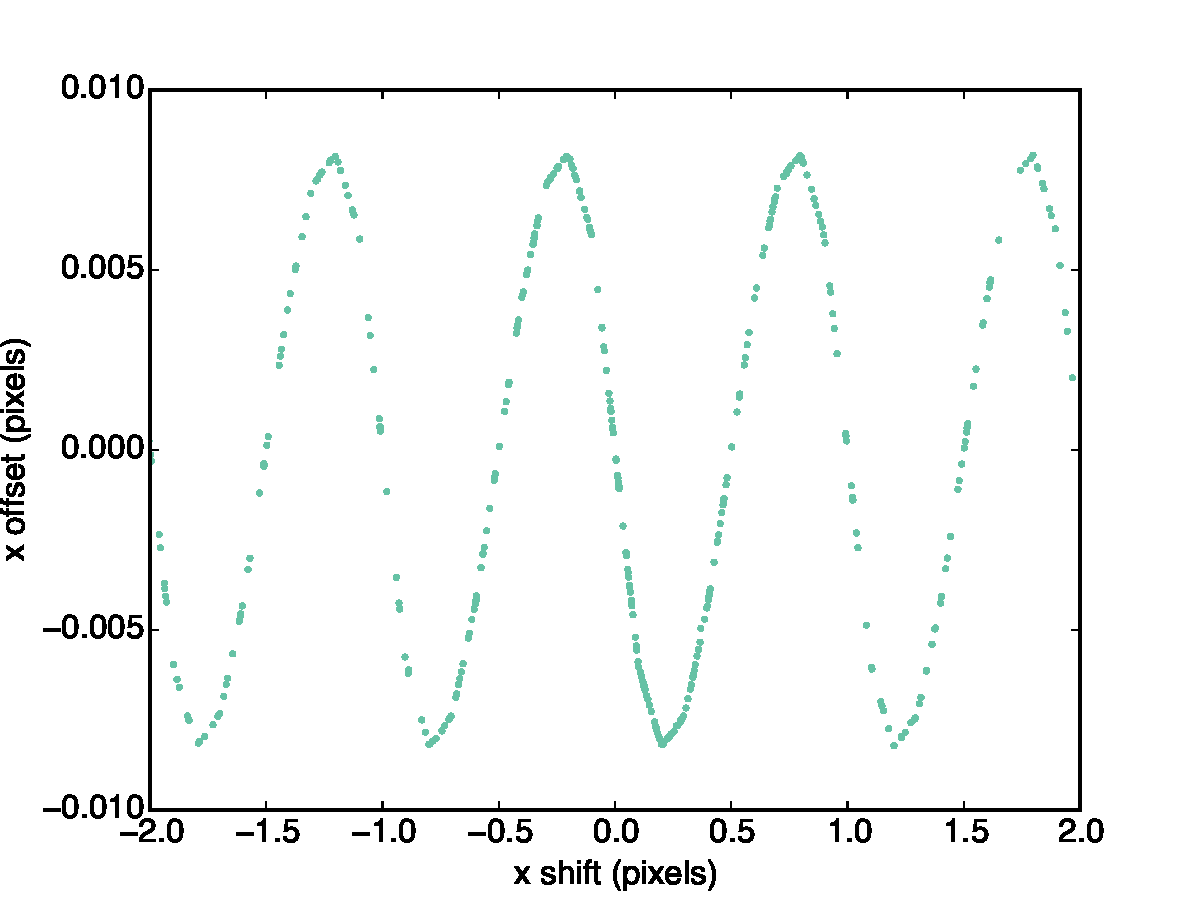
\includegraphics[width=0.8\textwidth]{crosscorr_cenWithNoise}
      \caption{offset for measured shift and real shift. Original
        image and shifted iamge were both added with 5 fake star in
        random poistions.}
      \label{fig:shift2}
    \end{figure}

 \section{PSF subtraction result}
Using cross correlation and  World Coordinate System to register
images, two set of data were compiled. I carried out the PSF
subtraction with both data set.\par

For one specific image(img$_{0}$), every other image(img$_{i}$) that was taken with the same
filter and different rolling angle were selected to be
subtracted. With equation \ref{eqn:fit}:
\begin{equation}
  \label{eqn:fit}
  res = \sum(img_{0} - c\cdot img_{i})^{2}
\end{equation}
tunable scale factor $c$ is calculated with minimum least square
fitting. The PSF is chosen with the criterion of least residual. \par

Figure \ref{fig:subcomp} illustrate the difference of PSF subtraction
results between cross correlation and WCS registration. It is clearly
shown that cross correlation gives a better alignment that the
residual image is much more even. WCS aligned PSF is clearly offset to
downright direction.\par

The background fluctuation of the region around secondary is $\sim
1.0$ counts/s.\par

\begin{figure}
  \centering
  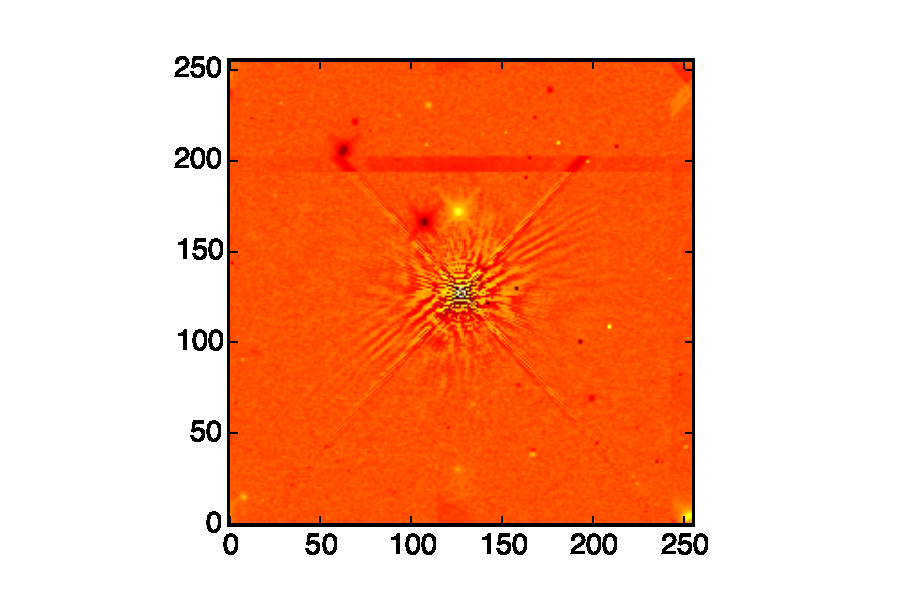
\includegraphics[width=\textwidth]{cc_example}
  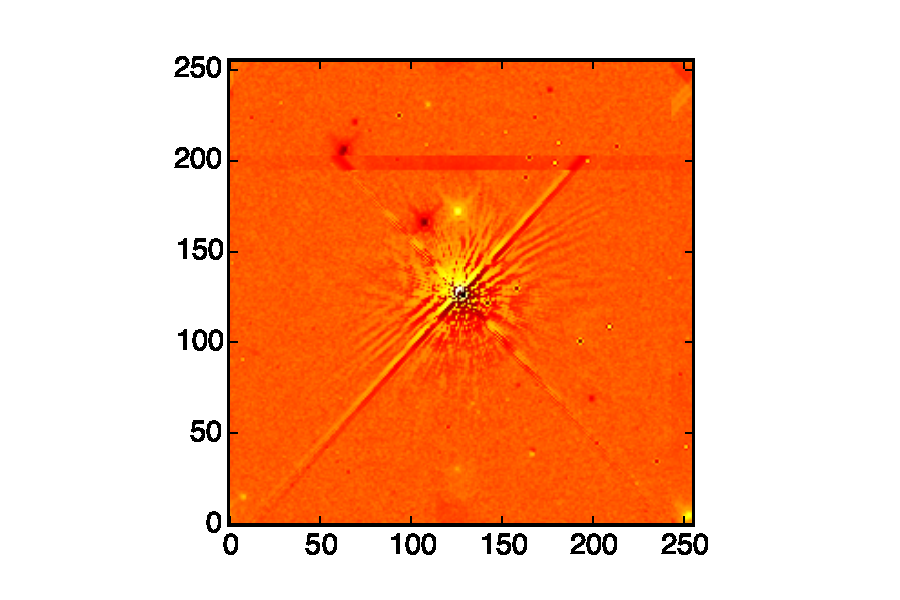
\includegraphics[width=\textwidth]{wcs_example}
  \caption{PSF subtraction comparison. Above: cross
    correlation. Below: WCS}\label{fig:subcomp}
\end{figure}
\section{Aperture Photometry Result}
\subsection{Light Curves}

The light curve measurements for both absolute fluxes and relative
fluxes are shown in Figure \ref{fig:lightcurve}. Figure
\ref{fig:glenn} is Glenn's preliminary measurements. The lower plot in
figure \ref{fig:lightcurve} is very similar to figure
\ref{fig:glenn}. However, in figure \ref{fig:glenn}, the light curves
for F125W and F160W show considerable discrepancies in 5th and 6th
orbits. However in my measurement, the two curves agree better. Apart
from this, the most prominent features are shown in both light
curves, e.g. the light curves are lower in 2nd orbit and the
discrepancy at start of the 3rd orbit.

\begin{figure}
  \centering
  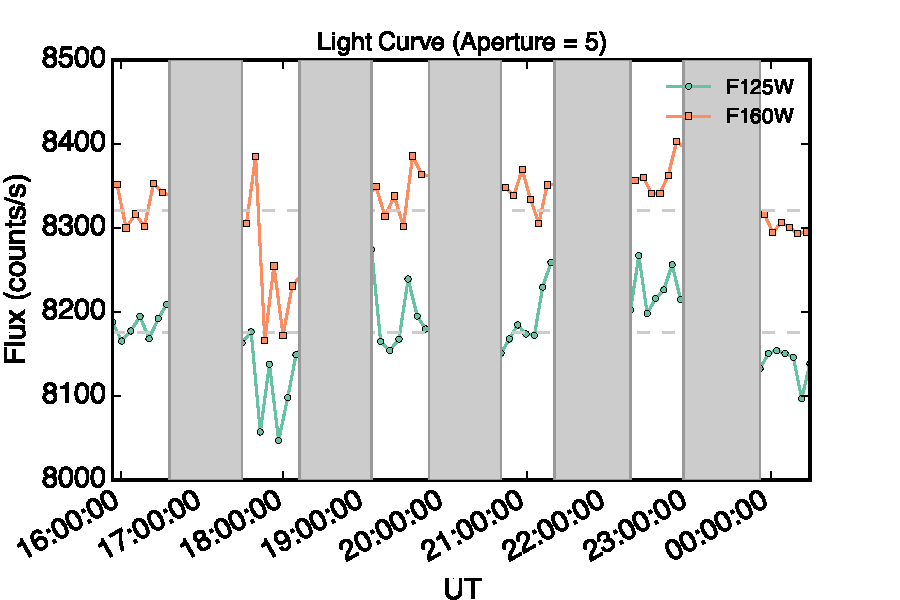
\includegraphics[width=0.8\textwidth]{fluxcurve_aper_05}
  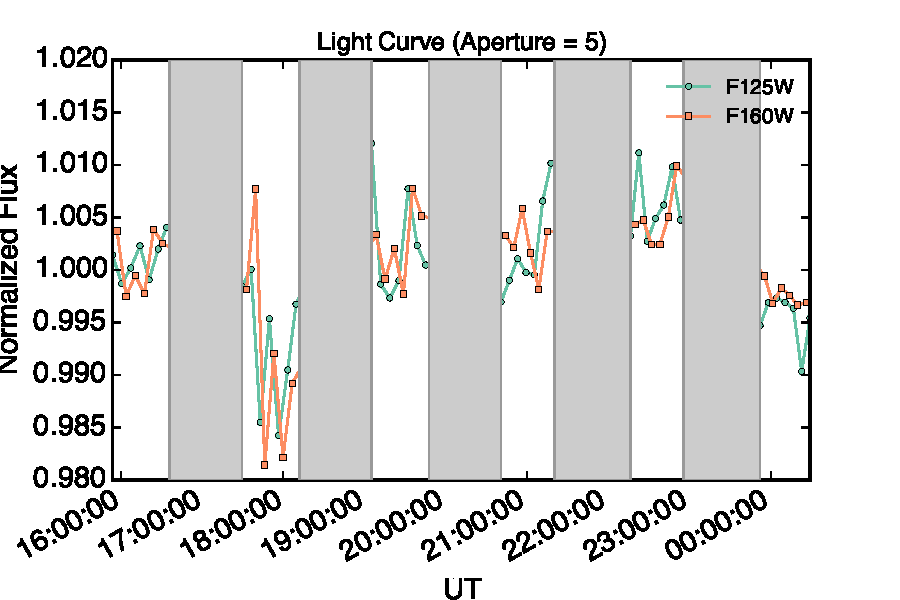
\includegraphics[width=0.8\textwidth]{relativefluxcurve_aper_05}
  \caption{Filter F125W and F160W light curves. Upper images shows the
    curve for absolute flux (count per second) changing with time. The
    mean values for both light curves are plotted with gray dashed
    lines. In the lower image, two light curves are normalized with
    the mean value of itself.}
  \label{fig:lightcurve}
\end{figure}

\begin{figure}
  \centering
    \centering
    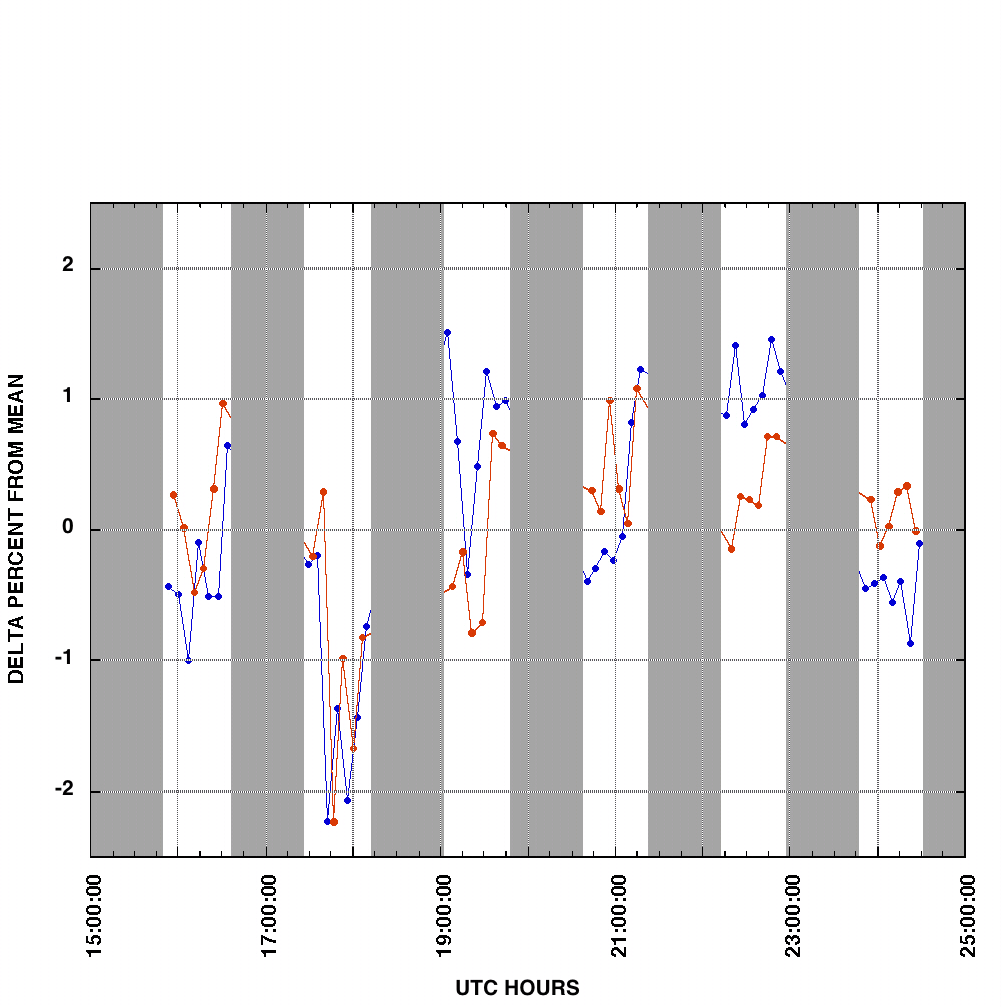
\includegraphics[width=0.8\textwidth]{ABPIC_DELTA_PERCENT_INITIAL}
    \caption{Glenn's preliminary measurement}
    \label{fig:glenn}
  \end{figure}

\subsection{Error Estimation}
Considering statistical uncertainty and fluctuation of background sky,
the relative error for one aperture photometry measurement is below
0.3\% according to my estimation. The error estimation procedure is
explained as following.\par

Statistical uncertainty:
\begin{equation}
  \sigma_{\mathrm{stat}}^{2}=ft_{\mathrm{expo}}
\end{equation}
Background fluctuation:
\begin{equation}
  \sigma_{\mathrm{sky}}^{2}=N\sigma_{\mathrm{sky,0}}^{2}t_{expo}
\end{equation}
Total error are the combination of these two parts:
\begin{equation}
  \sigma^{2} = \sigma_{\mathrm{stat}}^{2}+\sigma_{\mathrm{sky}}^{2}=ft_{\mathrm{expo}}+N\sigma_{\mathrm{sky,0}}^{2}t_{expo}
\end{equation}
Relative uncertainty:
\begin{equation}
  \frac{\sigma}{\mathrm{Flux}} = \frac{\sqrt{ft_{\mathrm{expo}}+N\sigma_{\mathrm{sky,0}}^{2}t_{expo}}}{ft_{\mathrm{expo}}}
\end{equation}
The exposure time are 30s for F125W images and 15s for F160W
images. Here I adopt 15s for a upper limit estimation. The flux
intensity for the exoplanet is $\sim 8000$ counts per second. The
standard deviation for background is $\sim 1$ counts per
second. Plugin those numbers, I estimated a relative uncertainty for 0.3\%.
\end{document}
%%% Local Variables:
%%% mode: latex
%%% TeX-master: t
%%% End:
